% \chapter{陽子--${}^3$He弾性散乱実験による${}^3$He偏極分解能測定}
% 1.2節で述べたように、我々のグループは中間エネルギー領域における陽子--$^3$Heの散乱系を系統的に調べていくために、陽子--$^3$He弾性散乱における完全測定を目標としている。そのために、東北大学サイクロトロンRIセンター(CYRIC)で陽子--$^3$He弾性散乱実験を行い、有効散乱角度における$^3$He偏極分解能の測定を行った。陽子ビームの入射エネルギーは、中間エネルギー領域である$70~{\rm MeV}$とした。$^3$He偏極分解能の測定には偏極$^3$He標的の偏極度の絶対値を知る必要がある。$^3$He偏極度の絶対値は、本研究において開発したRbのESR周波数シフト測定システムによって、実験中に測定したNMR信号を較正することで得られる。\\
%  本章では、$^3$He偏極分解能測定のために2015年10月に東北大学CYRICで行った$70~{\rm MeV}$の陽子ビームを用いた陽子--偏極$^3$He弾性散乱実験について述べる。

% %%%% 5.1 %%%%
%  \section{実験概要}
% 実験は東北大学CYRICの41コースビームライン(第四ターゲット室)で行った。イオン源で生成された陽子ビームはAVFサイクロトロンによって加速され、第四ターゲット室まで輸送される。偏極$^3$He標的は第四ターゲット室に置かれている散乱槽の下流に設置した。またその下流に、ビームを止めかつその電流値を測定するためにファラデーカップ(F.C.)を設置した。またビームの入射方向に対して左右それぞれに検出器を設置し、散乱陽子を検出した。実験中はAFP-NMR法によって$^3$He原子核の核スピンの反転および$^3$He偏極度の測定を行った。$^3$Heの偏極方向の反転前後における散乱陽子の検出数を比較し、その非対称度から$^3$He偏極分解能を求める。また散乱槽内にはターゲットラダーが設置されており、ラダーに厚さ$20~{\rm \mu m}$のポリエチレンフィルムを取り付けた。ポリエチレンと衝突した散乱陽子を散乱槽内に設置した検出器で検出し、ビーム強度のモニターを行った。散乱槽は、真空引きを行い$\sim 10^{-3}~{\rm Pa}$程度の真空状態とした。散乱実験時の検出器系の概観図を図\ref{exp_setup}に示す。

% \begin{figure}[tbp]
%  \centering
%  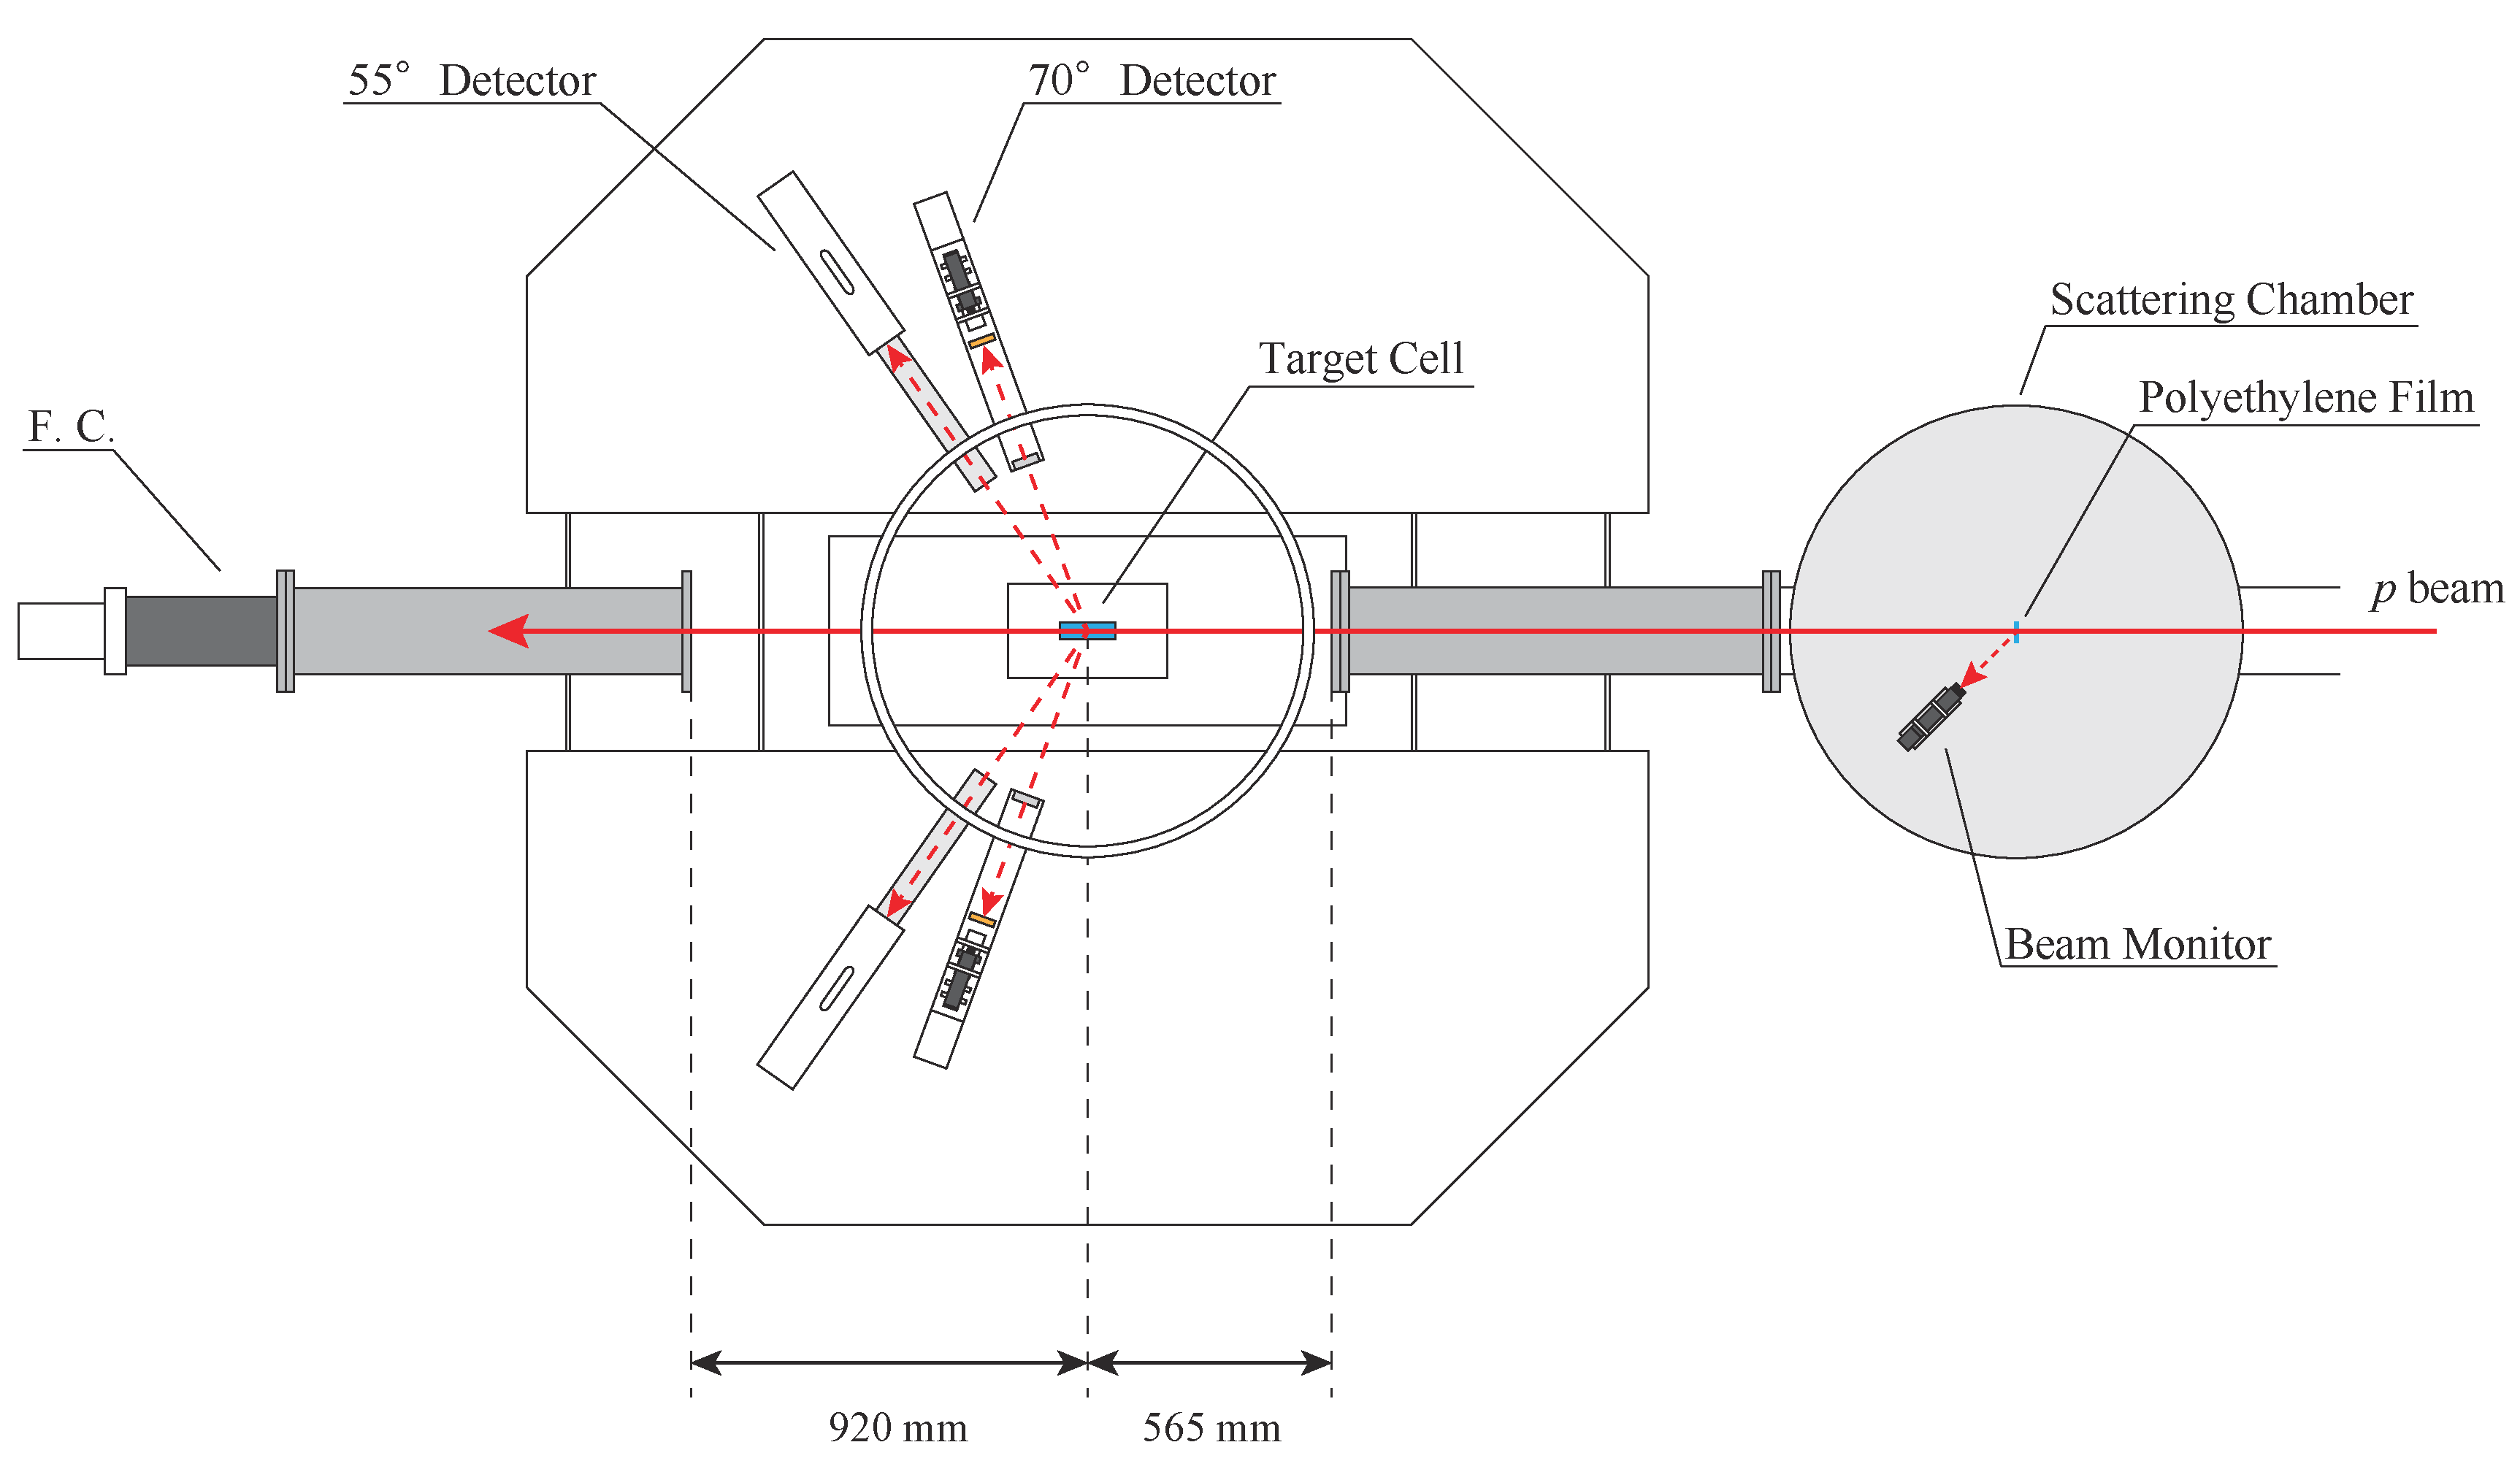
\includegraphics[clip, width=1.0\linewidth]{./chap5/fig/cyric_exp_setup2.pdf}\\
%  \caption{散乱実験における検出器系の概観図}
%  \label{exp_setup}
% \end{figure}

% %%%%%%%%%%

% %%%% 5.2 %%%%
%  \section{検出器系および標的}
% $^3$Heと弾性散乱した陽子の検出は、ビーム方向に対して左右それぞれに実験室系での散乱角度$55^{\circ}$および$70^{\circ}$に設置した検出器によって行った。また散乱槽内には陽子ビームの強度をモニターするために検出器を設置した。以下の節では、これらの検出器および今回の実験で使用した散乱標的について述べる。

% %% 5.2.1 %%
%   \subsection{$55^{\circ}$検出器}
% $^3$Heと弾性散乱した散乱陽子を検出するために、偏極$^3$He標的の周りに架台を設置し、その上に検出器を設置した。ビーム方向に対して左右それぞれについて実験室系での角度$55^{\circ}$に設置した検出器は、プラスチックシンチレーターと光電子増倍管(PMT)を光学的に接着したものから構成される。実験室系での散乱角度$55^{\circ}$に設置した検出器の概形を図\ref{55detect}に、またその仕様を表\ref{55detect_design}に示す。検出器はエネルギー損失用の$dE$検出器と全エネルギー検出用の$TE$検出器とを組み合わせたものである。これらの検出器の前方には、標的セルのガラスの入射部分および出射部分から散乱された陽子を遮蔽するために厚さ$20~{\rm mm}$のアルミ製筒型コリメーターが設置されている。散乱陽子のイベントは$dE$および$TE$検出器からの信号のコインシデンスを取ることで取得した。

% \begin{figure}[tbp]
%  \centering
%  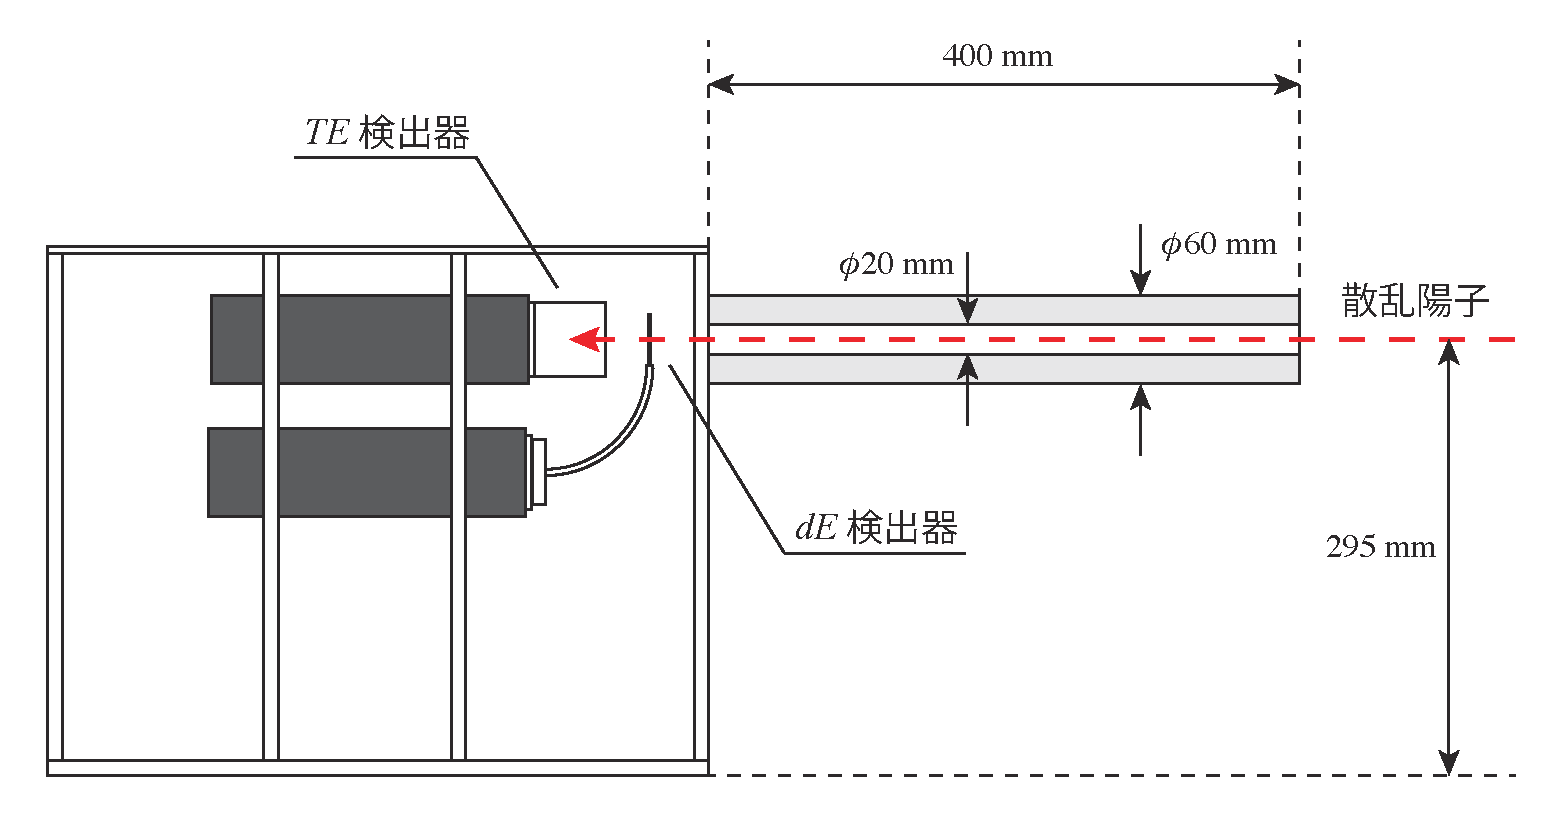
\includegraphics[clip, width=11cm]{./chap5/fig/p-detector_55.pdf}\\
%  \caption{実験室系の散乱角度$55^{\circ}$に設置した検出器の概形}
%  \label{55detect}
% \end{figure}

% \begin{table}[htbp]
%  \caption{$55^{\circ}$検出器の仕様}
%  \centering
%   \begin{tabular}{|c||c|c|} \hline
%  & $dE$検出器 & $TE$検出器 \\ \hline
%  シンチレーター & BC-408 & BC-408 \\
%  厚さ & $1~{\rm mm}$ & $50~{\rm mm}$ \\
%  寸法 & $40~{\rm mmW} \times 40~{\rm mmH}$ & $\phi 50~{\rm mm}$ \\
%  PMT & H1161 & H1161 \\ \hline
%   \end{tabular}
%  \label{55detect_design}
% \end{table}
% %
% シンチレーターを荷電粒子が通過すると、シンチレーター内の電子と荷電粒子が電磁相互作用を起こし、シンチレーター中の分子が励起される。励起状態の分子はやがて光子を放出して基底状態へと脱励起する。この時放出される光子数(蛍光強度)は、荷電粒子がシンチレーター中で失ったエネルギーに比例する。シンチレーターから放出された光子は、PMTによって電気信号に変換され、増幅される。PMTが出力する信号強度は、入射光子数に比例し、またPMTの電極に印加される高電圧のべき乗に比例する。よって、最終的にPMTから得られる電気信号強度は、荷電粒子がシンチレーター内で損失したエネルギーに比例することになる。

% %%%%%%%

% %% 5.2.2 %%
%   \subsection{$70^{\circ}$検出器}
% ビーム方向に対して、左右それぞれについて実験室系での散乱角度$70^{\circ}$にも検出器を設置した。これらの検出器は、プラスチックシンチレーターとPMTを光学的に接着した$dE$検出器と、NaIシンチレーターとPMTを光学的に接着した$TE$検出器から構成される。実験室系での散乱角度$70^{\circ}$に設置した検出器の概形を図\ref{70detect}に、またその仕様を左側および右側に設置した検出器それぞれについて表\ref{l70detect_design}および表\ref{r70detect_design}に示す。$55^{\circ}$検出器と同様に、標的セルのガラスの入射部分および出射部分から散乱された陽子を遮蔽するために厚さ$20~{\rm mm}$のジュラルミン製の板を前方に設置し、検出器の直前に厚さ$15~{\rm mm}$の真鍮の板を設置した。散乱陽子のイベントは、$55^{\circ}$検出器と同様に$dE$および$TE$検出器からの信号のコインシデンスを取ることで取得した。

% \begin{figure}[tbp]
%  \centering
%  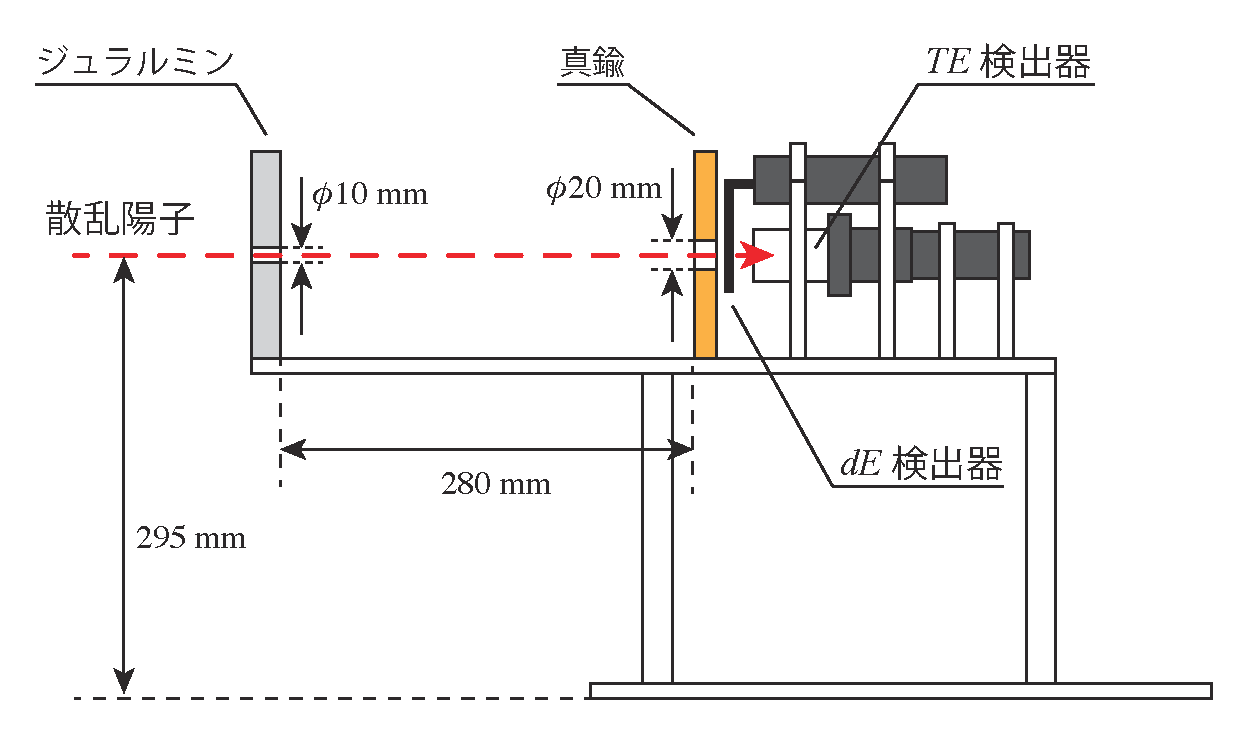
\includegraphics[clip, width=9cm]{./chap5/fig/p-detector_70.pdf}\\
%  \caption{実験室系の散乱角度$70^{\circ}$に設置した検出器の概形}
%  \label{70detect}
% \end{figure}

% \newpage
% \begin{table}[htbp]
%  \caption{左側の$70^{\circ}$検出器の仕様}
%  \centering
%   \begin{tabular}{|c||c|c|} \hline
%  & $dE$検出器 & $TE$検出器 \\ \hline
%  シンチレーター & BC-408 & NaI \\
%  厚さ & $2~{\rm mm}$ & $30~{\rm mm}$ \\
%  寸法 & $30~{\rm mmW} \times 65~{\rm mmH}$ & $30~{\rm mmW} \times 30~{\rm mmH}$ \\
%  PMT & H7415MOD & H7415MOD \\ \hline
%   \end{tabular}
%  \label{l70detect_design}
% \end{table}
% %
% \begin{table}[htbp]
%  \caption{右側の$70^{\circ}$検出器の仕様}
%  \centering
%   \begin{tabular}{|c||c|c|} \hline
%  & $dE$検出器 & $TE$検出器 \\ \hline
%  シンチレーター & BC-408 & NaI \\
%  厚さ & $0.5~{\rm mm}$ & $30~{\rm mm}$ \\
%  寸法 & $25~{\rm mmW} \times 25~{\rm mmH}$ & $30~{\rm mmW} \times 30~{\rm mmH}$ \\
%  PMT & H7415MOD & H7415MOD \\ \hline
%   \end{tabular}
%  \label{r70detect_design}
% \end{table}
% %

% %%%%%%%

% %% 5.2.3 %%
%   \subsection{ビームモニター}
% 散乱実験中のビーム強度をモニターするために、偏極$^3$He標的の上流に設置されている散乱槽内にビームモニターを設置した。ビームモニターは、プラスチックシンチレーターとPMTを光学的に接着したものから構成される。$55^{\circ}$検出器および$70^{\circ}$検出器同様、ビームモニターはエネルギー損失用の$dE$検出器と全エネルギー検出用の$TE$検出器とを組み合わせたものである。散乱槽内に設置したビームモニターの概形を図\ref{BM}に、またその仕様を表\ref{BM_design}に示す。散乱槽内のラダーに取り付けられた厚さ$20~{\rm \mu m}$のポリエチレンフィルムによって散乱された陽子を、$dE$および$TE$検出器からの信号のコインシデンスを取ることでイベントとして取得した。また、ビームモニターは実験室系での散乱角度$45^{\circ}$に設置し、ポリエチレン標的から$TE$検出器のNaIシンチレーターの入射面までの距離を$190~{\rm mm}$とした。

% \begin{figure}[tbp]
%  \centering
%  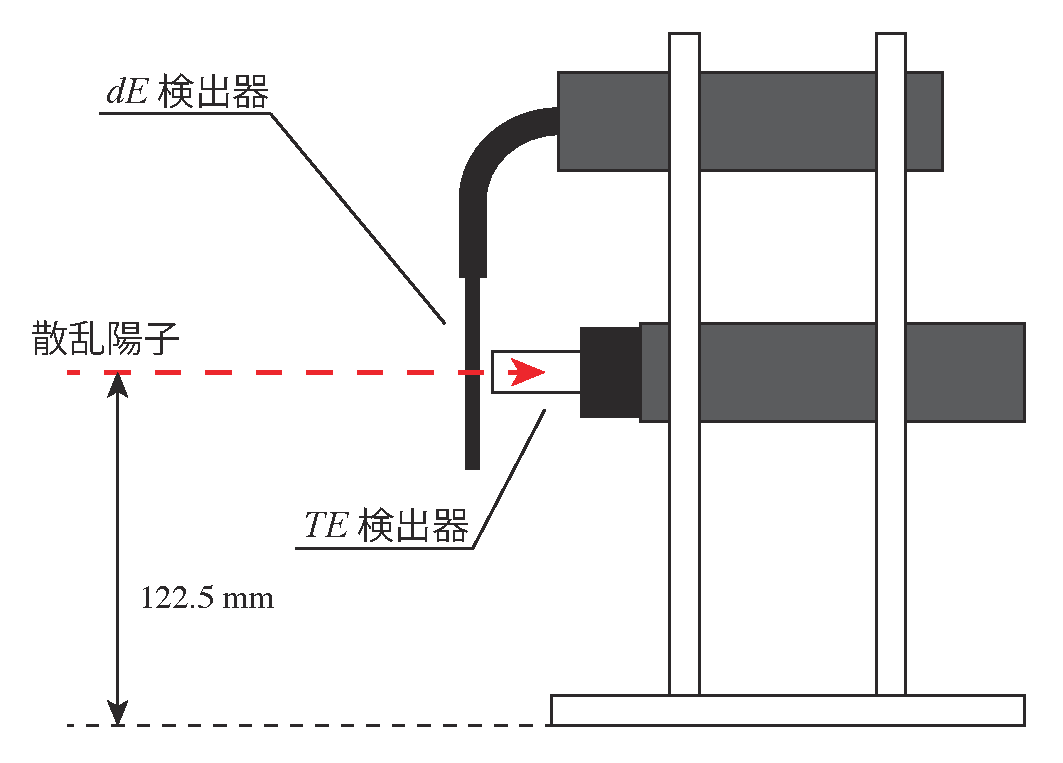
\includegraphics[clip, width=7.5cm]{./chap5/fig/beam_monitor.pdf}\\
%  \caption{散乱槽内に設置したビームモニターの概形}
%  \label{BM}
% \end{figure}

% \begin{table}[htbp]
%  \caption{ビームモニターの仕様}
%  \centering
%   \begin{tabular}{|c||c|c|} \hline
%  & $dE$検出器 & $TE$検出器 \\ \hline
%  シンチレーター & BC-408 & NaI \\
%  厚さ & $2~{\rm mm}$ & $35~{\rm mm}$ \\
%  寸法 & $35~{\rm mmW} \times 65~{\rm mmH}$ & $\phi 14~{\rm mm}$ \\
%  PMT & H7415MOD & H7415MOD \\ \hline
%   \end{tabular}
%  \label{BM_design}
% \end{table}
% %
% 散乱陽子の検出数はビーム強度に比例するので、全検出数からビーム強度の相対値が得られる。F.C.はその上流に空気や標的セル等が存在するため、ビーム強度が減衰していることが考えられる。よって、以下の解析でのビーム強度は、ビームモニターで得られた散乱陽子の検出数を用いた。

% %%%%%%%

% %% 5.2.4 %%
%   \subsection{散乱標的}
% 散乱実験時の偏極$^3$He標的の周囲の環境について述べる。図\ref{exp_setup}のように、偏極$^3$He標的は散乱槽の下流に設置した。標的セルとしては、3.1.2節の手順で作成したKukiセルを用いた。標的セルは大気中に設置されており、標的セルの中心から散乱槽のダクト出口部分までの距離は$565~{\rm mm}$とした。散乱槽のダクト出口部分は、厚さ$50~{\rm \mu m}$のカプトン膜が貼られたフランジが取り付けられており、これによって散乱槽内の真空を維持した。また、標的下流に設置されているF.C.のダクト入口部分から標的セルの中心までの距離は$920~{\rm mm}$とした。F.C.のダクトにもカプトン膜が貼られたフランジを取り付けた。


% %%%%%%%

% %%%%%%%%%%

% \newpage
% %%%% 5.3 %%%%
%  \section{実験条件}
% 今回行った散乱実験の条件を表\ref{exp_cond}に示す。また、散乱陽子を検出する各検出器についての条件も表\ref{detector_cond}に示す。
% %
% \begin{table}[htbp]
%  \caption{$70~{\rm MeV}$の陽子--偏極$^3$He弾性散乱実験の条件}
%  \centering
%   \begin{tabular}{|c|c|} \hline
% 入射ビーム & $70~{\rm MeV}$の陽子 \\
% ビーム強度 & 最大$12~{\rm nA}$ \\
% 標的 & $3$気圧の偏極$^3$Heガス ($3.68 \times 10^{-4}~{\rm g/cm^{3}}$) \\
% 検出器設置角度 & $55^{\circ}$, $70^{\circ}$(実験室系)\\
% ビームモニター用標的 & ポリエチレン(厚さ$20~{\rm \mu m}$) \\
% ビームモニター設置角度 & $45^{\circ}$(実験室系) \\ \hline
%   \end{tabular}
%  \label{exp_cond}
% \end{table}
% %
% \begin{table}[htbp]
%  \caption{各検出器の条件。PSはプラスチックシンチレーターを表す。}
%  \centering
%   \begin{tabular}{|c||c|c|c|} \hline
%  & $55^{\circ}$検出器 & $70^{\circ}$検出器 & ビームモニター \\ \hline
%  $dE$検出器 & PS+PMT & PS+PMT & PS+PMT \\
%  $TE$検出器 & PS+PMT & NaI+PMT & NaI+PMT \\
%  厚さ($dE$検出器) & $1~{\rm mm}$ & $2~{\rm mm}$, $0.5~{\rm mm}$ & $2~{\rm mm}$ \\
%  厚さ($TE$検出器) & $50~{\rm mm}$ & $30~{\rm mm}$ & $35~{\rm mm}$ \\
%  標的中心から$TE$検出器までの距離 & $880~{\rm mm}$ & $750~{\rm mm}$ & $210~{\rm mm}$ \\
%  立体角 & $0.5~{\rm msr}$ & $0.43~{\rm msr}$ & $4.3~{\rm msr}$ \\ \hline
%   \end{tabular}
%  \label{detector_cond}
% \end{table}
% %

% %%%%%%%%%%

% \newpage
% %%%% 5.4 %%%%
%  \section{測定および解析結果}
% 本実験で得られた測定結果から、陽子--$^3$He弾性散乱起因のイベントを選び出すための解析方法、およびその解析結果について述べる。

% %% 5.4.1 %%
%   \subsection{陽子--$^3$He弾性散乱イベントの抽出}
% 実験室系での散乱角度$55^{\circ}$に設置した左側の$dE$検出器および$TE$検出器で得られた典型的なADCスペクトルの二次元相関図を図\ref{L55_ADC2D}に示す。横軸が$dE$検出器のchannel(以下、chと表記)であり、縦軸が$TE$検出器のchである。$55^{\circ}$検出器での二次元ADCスペクトルにおいて、横軸$180~{\rm ch}$、縦軸$900~{\rm ch}$付近に見られるピークが$^3$He原子核と弾性散乱した陽子によるものである。

% \begin{figure}[htbp]
%  \centering
%  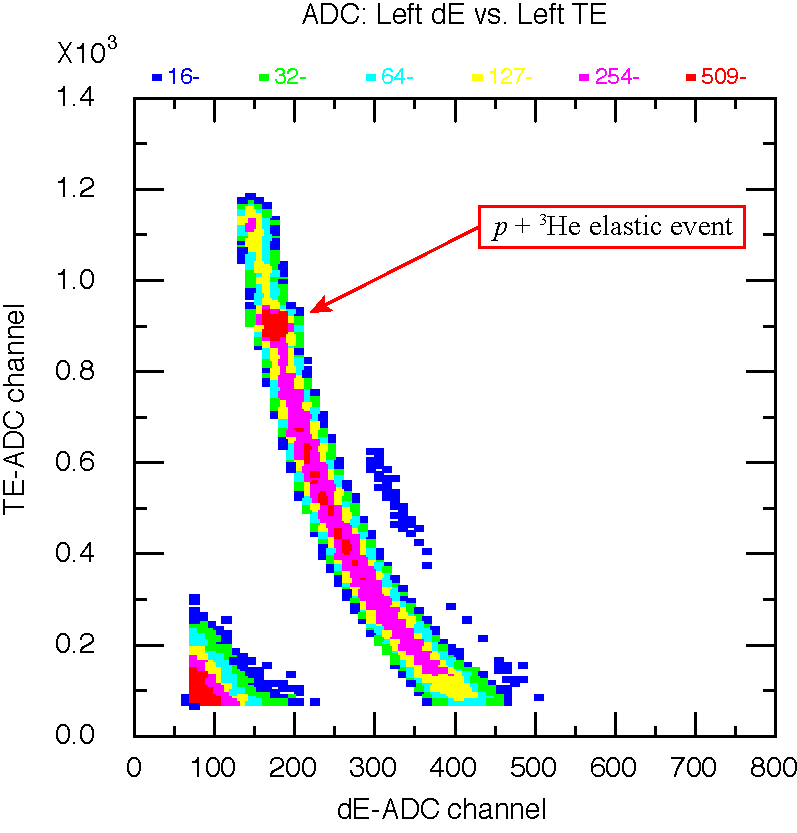
\includegraphics[clip, width=7cm]{./chap5/fig/L55ADC2D_203_cl.pdf}\\
%  \caption{左側の$55^{\circ}$検出器の二次元ADCスペクトル}
%  \label{L55_ADC2D}
% \end{figure}

% 得られたADCスペクトルから、陽子--$^3$He弾性散乱イベントの検出数を求める。$55^{\circ}$検出器の$TE$検出器で得られた一次元ADCスペクトルを図\ref{L55_TEADC}に示す。検出数は、図\ref{L55_TEADC}における点線で囲われたピーク部分を数えることで得た。同様に、他の検出器についても陽子--$^3$He弾性散乱イベントの検出数を求めた。この時、検出数を得る時の$TE$検出器のADCスペクトルのch幅は$100~{\rm ch}$となるようにした。

% \begin{figure}[tbp]
%  \centering
%  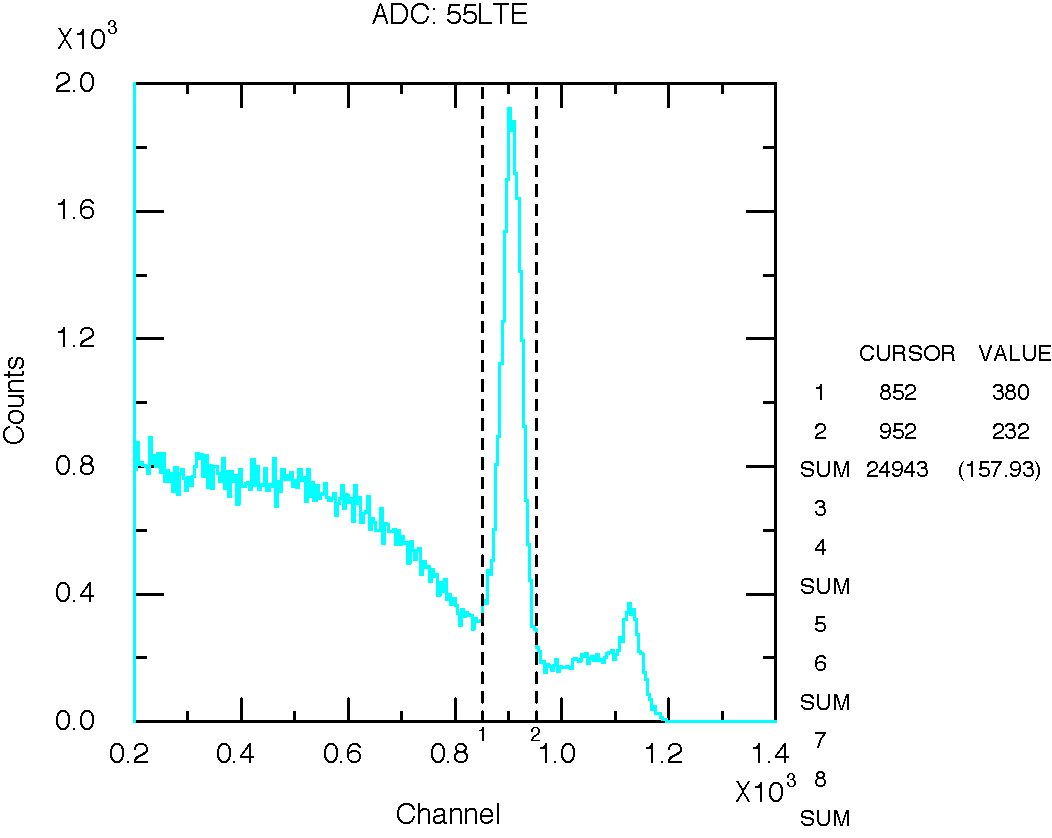
\includegraphics[clip, width=9cm]{./chap5/fig/L55TEADC_203_2.pdf}\\
%  \caption{左側の$55^{\circ}$検出器の$TE$検出器の一次元ADCスペクトル}
%  \label{L55_TEADC}
% \end{figure}

% %%%%%%%

% %% 5.4.2 %%
%   \subsection{バックグラウンドの評価}
% $^3$He偏極分解能$A_y$は、式(\ref{Ay_calc})でも示したように
% %
%  \begin{equation}
%   A_y=\frac{1}{p_y} \frac{L_{\rm up}-L_{\rm down}}{L_{\rm up}+L_{\rm down}}=\frac{1}{p_y} \frac{R_{\rm down}-R_{\rm up}}{R_{\rm up}+R_{\rm down}}
%   \label{Ay_calc2}
%  \end{equation}
%  %
% と表される。ここで、$L$および$R$は検出器での散乱陽子の検出数を入射ビーム強度で規格化したものを表す。$^3$He偏極分解能$A_y$は$^3$Heの核スピンの反転前後で得られた検出数の差を、その和で割ることで計算される。しかし、上記の方法で得た検出数はいくらかのバックグラウンドを含んでいる。よって、式(\ref{Ay_calc2})において検出数の差を取る分子ではバックグラウンドが打ち消されるが、検出数の和を取る分母ではバックグラウンドも足されるので、結果的に$^3$He偏極分解能$A_y$の値が小さくなってしまう。故に、式(\ref{Ay_calc2})における分母の検出数$L$, $R$は、バックグラウンドを除いた検出数$L'$, $R'$である必要がある。\\
% 得られたADCスペクトルにおけるバックグラウンドを見積もるために、$^3$Heガス、N$_2$ガスおよびRbを含まないブランクセルを用いた測定を行った。ブランクセルは、Kukiセルと同様の手順で洗浄を行い、最後にガスを封入せず真空引きのみを行って封じ切った“Koga”セルを用いた。\\
%  ブランクセルによる測定で得られたADCスペクトルを用いて、各検出器における一次元ADCスペクトルのバックグラウンドを取り除く。図\ref{L55_TEADC_bg}にバックグラウンドを差し引く前後における左側の$55^{\circ}$検出器の$TE$検出器における一次元ADCスペクトルを示す。図\ref{L55_TEADC_bg}において、点線で囲われた部分を陽子--$^3$He弾性散乱イベントの検出数として取得した。この時、点線で囲われた部分の幅は$100~{\rm ch}$とした。

% \begin{figure}[tbp]
%  \centering
%  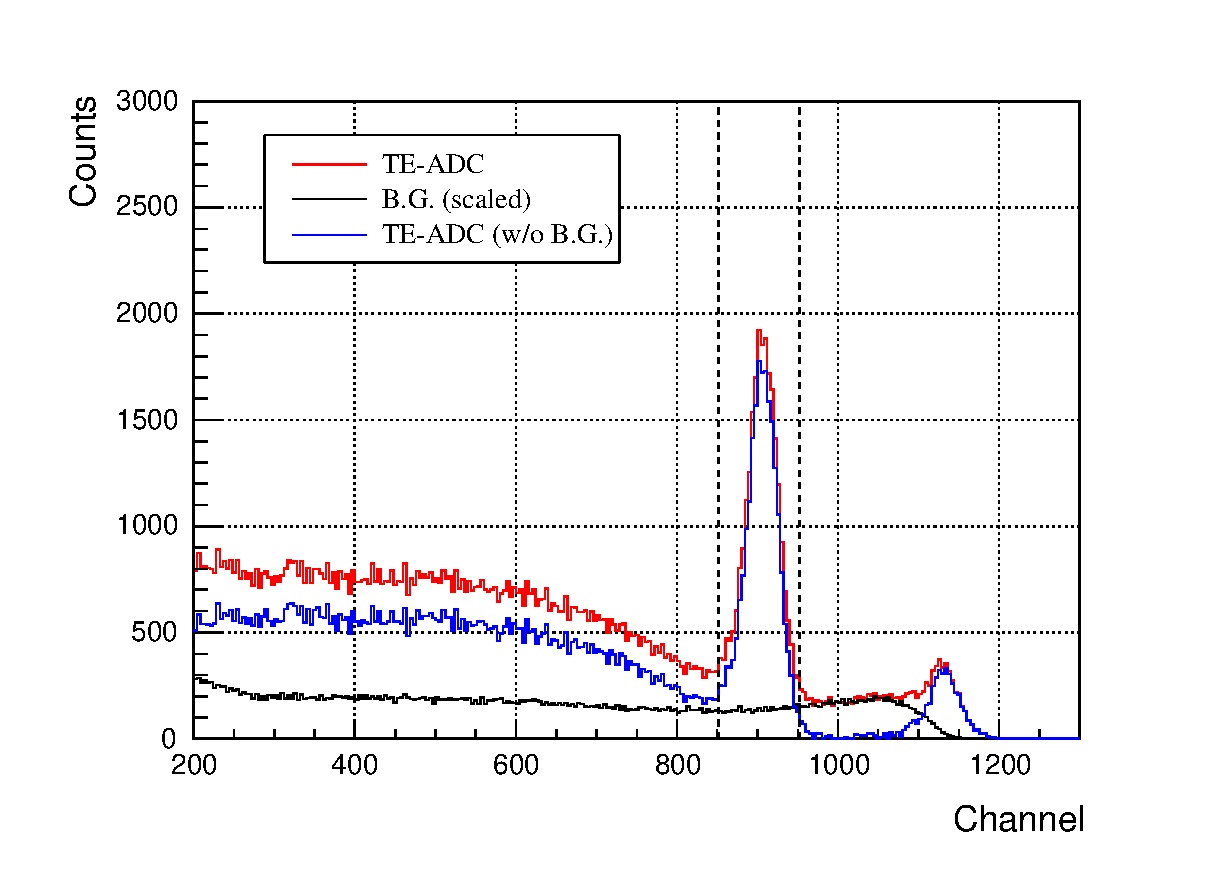
\includegraphics[clip, width=10cm]{./chap5/fig/L55TEADC_203_bg2.eps}\\
%  \caption{左側の$55^{\circ}$検出器の$TE$検出器の一次元ADCスペクトル。黒線のB.G.を赤線のADCスペクトルから差し引いた。}
%  \label{L55_TEADC_bg}
% \end{figure}

% %%%%%%%

% %% 5.4.3 %%
%   \subsection{解析結果}
% 前述の解析方法によって求めた陽子--$^3$He弾性散乱イベントの検出数、また実験中に得られたNMR信号強度によって求められた$^3$He偏極度を用いて、$^3$He偏極分解能$A_y$を求めた。本節では、これらの解析結果について述べる。\\
%  5.4.1節で述べた方法で求めた陽子--$^3$He弾性散乱イベントの検出数を、ビームモニターでの散乱陽子の検出数と検出器での検出効率の積で割った結果を図\ref{Yield_55}および図\ref{Yield_70}に示す。$55^{\circ}$検出器については図\ref{Yield_55}に、また$70^{\circ}$検出器については図\ref{Yield_70}に示している。図\ref{Yield_55}および図\ref{Yield_70}において、横軸はRun番号を示す。偏極$^3$He原子核の核スピンの向きによって検出数に非対称度が現れていることが分かる。また実験中にAFP-NMR法によって測定したNMR測定結果を図\ref{Vnmr_exp}に示す。横軸は実験開始時を$0~{\rm hour}$とした時の時間で、縦軸はNMR信号強度である。更に図\ref{Vnmr_exp}では、本研究で開発したRbのESR周波数シフト測定システムによって較正したNMR信号強度に対する$^3$He偏極度$P_{\rm ^3He}$も右側の縦軸に示しており、またビームが標的に照射されている時間を赤い帯で示している。各Runの前後で得られたNMR信号強度から、式(\ref{rel_P_3He-Vnmr})を用いて$^3$He偏極度$p_y$を求めた。Run中における$^3$He偏極度は、Run前後で得られた値の平均値とした。本実験における典型的な$^3$He偏極度は$11$%程度であった。

% \begin{figure}[tbp]
%  \centering
%  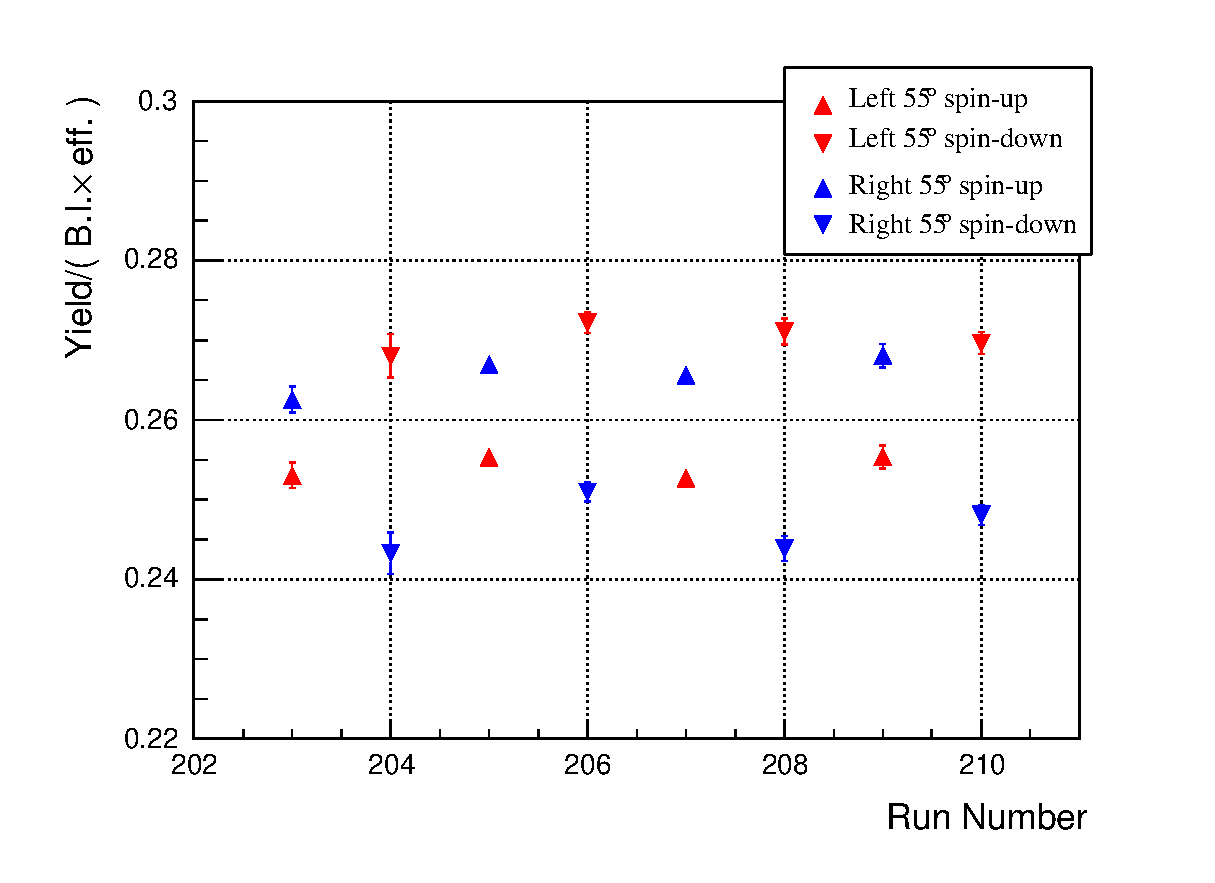
\includegraphics[clip, width=10cm]{./chap5/fig/asym_55deg.eps}\\
%  \caption{$55^{\circ}$検出器での散乱陽子の検出数とビーム強度および検出効率との比}
%  \label{Yield_55}
% \end{figure}

% \begin{figure}[tbp]
%  \centering
%  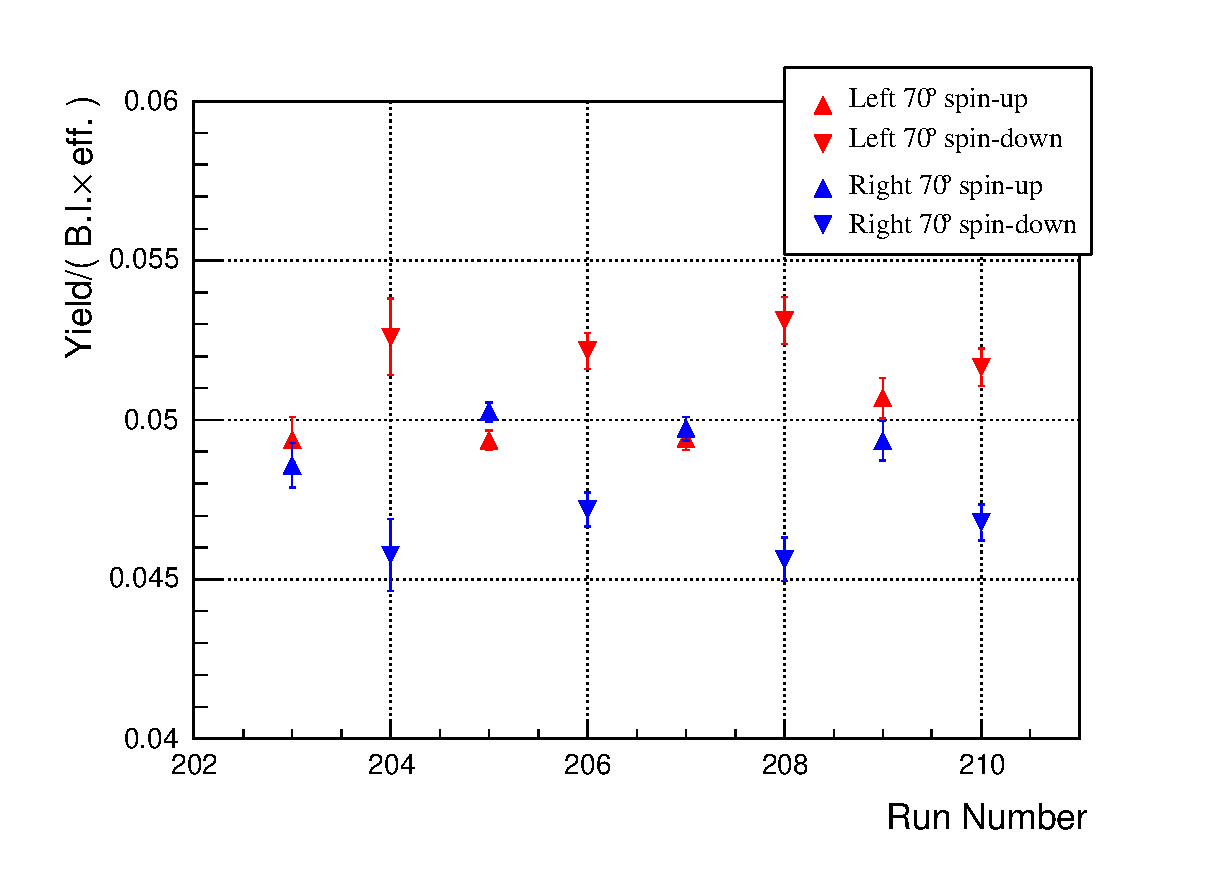
\includegraphics[clip, width=10cm]{./chap5/fig/asym_70deg.eps}\\
%  \caption{$70^{\circ}$検出器での散乱陽子の検出数とビーム強度および検出効率との比}
%  \label{Yield_70}
% \end{figure}

% \begin{figure}[tbp]
%  \centering
%  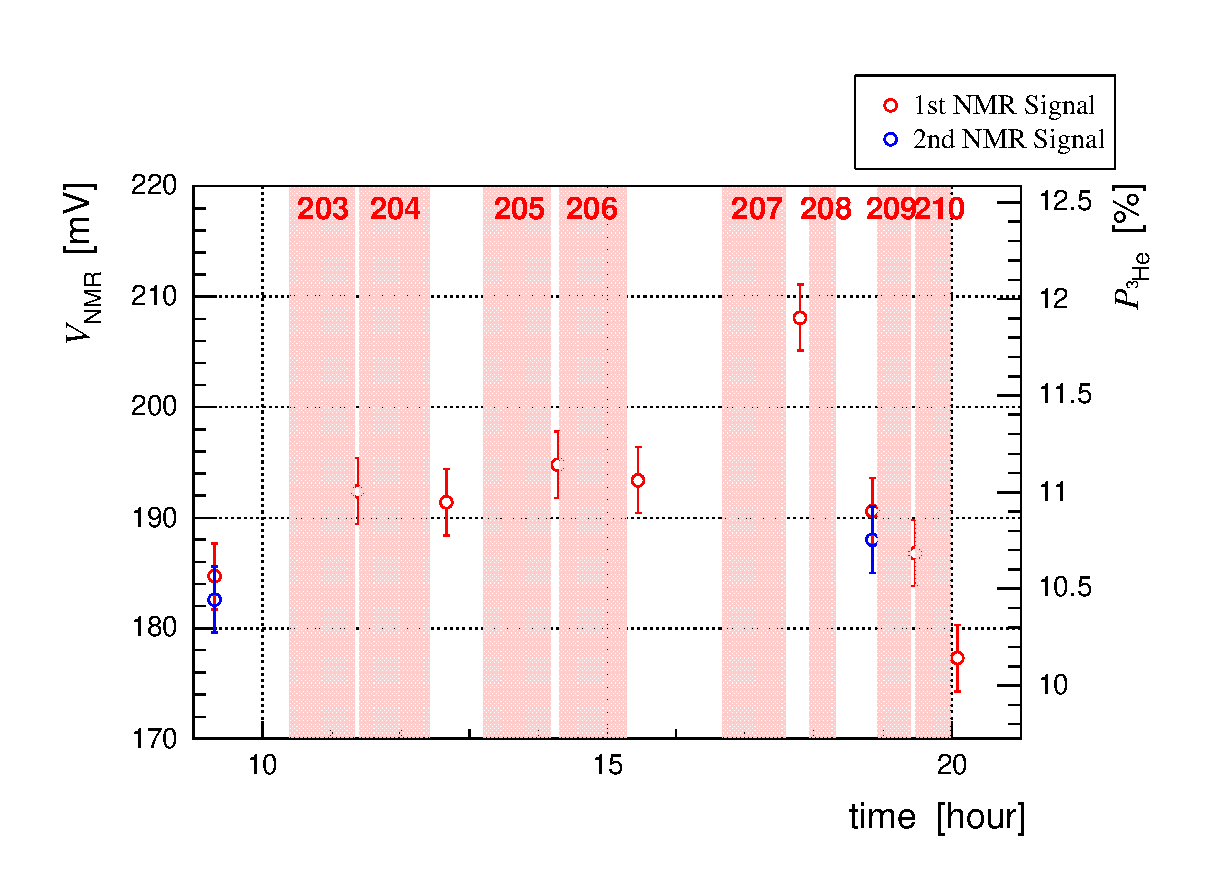
\includegraphics[clip, width=11cm]{./chap5/fig/Vnmr_oct15cyric_70.eps}\\
%  \caption{散乱実験中のNMR信号の推移。ビーム照射中を表す赤い帯の上部にRun番号を示した。}
%  \label{Vnmr_exp}
% \end{figure}


% 以上の手順によって陽子--$^3$He弾性散乱イベントの検出数および$^3$He偏極度$p_y$を求め、それら値を式(\ref{Ay_calc2})に代入することで$^3$He偏極分解能$A_y$を求めた。この時、陽子--$^3$He弾性散乱イベントの検出数を、ビームモニターでの散乱陽子の検出数と検出器での検出効率の積で割った値を用いた。また式(\ref{Ay_calc2})における分母の検出数は、バックグラウンドを差し引いた値を用いた。更に、$^3$He偏極分解能$A_y$を求める際は他のRunから得られた検出数の重みつき平均をとって求めた。その結果、実験室系における散乱角度$\theta_{\rm lab} = 55^{\circ}$および$\theta_{\rm lab} = 70^{\circ}$における$^3$He偏極分解能$A_y$は
% %
% \begin{eqnarray}
%  A_y(\theta_{\rm lab} = 55^{\circ}) &=& -0.35 \pm (0.01)_{\rm stat}
%  \label{Ay_result_55} \\
%  A_y(\theta_{\rm lab} = 70^{\circ}) &=& -0.33 \pm (0.03)_{\rm stat}
%  \label{Ay_result_70}
% \end{eqnarray}
% %
% と求められた。ここで、$A_y$の誤差は統計誤差のみを示している。

% %%%%%%%

% %%%%%%%%%%
